
\chapter{Introduction to Signals and Systems}

\section{What is A Signal?}

\subsection{Definition of Signals}
The ``signal'' and ``system'' we study in this course is very prevelant to the design of real-world electronic devices.
But, before beginning to study them, we should first strive to understand their conceptual existence.

A signal is a conveyor of information. So, a signal is the transformation between a ``thing'' and a quantification of it.
In a biological perspective, any stimuli is a signal, because it delivers some information to our cognitive devices.
However, signals alone cannot alert or notify a cognitive device to perform some task, and we must therefore need another processor that can convert the signal into something else, or elicit information from a signal.
For example, just seeing the color on a red sign will not make you think that what lies beyond that sign must be suspicious; or, just seeing the color red will not make you think of the Hit Game Among Us.
There must be some other level of processes that picks up this color red, and performs some black-boxed operations to translate the signal of color red into ``danger!'', ``warning!'', ``Among Us!''
In a similar way, just receiving electronic waves is not sufficient for a machine to move. A machine must also be equipped with some other mechanism to interpret this electronic wave and its properties.

The process that generates or transforms signals into forms that we can understand or interpret is called a ``system''. In the formerly addressed biology case, your brain is a huge system.

\subsection{Abstraction of Signals}
Now that we have understood the layers of abstractions that signals and systems can be understood at, let's attempt at their mathematical representations.
Previously we addressed that a signal is a stimuli.
Now, imagine a waveform, a sound wave, such as the sound of a violin. The sound of a violin is the result of vibrating air, but that has no detectable mathematical formalism until we attempt to visualize a soundwave as a function.
In such case, the signal of violin sound maps the sound of violin per se, which has many original interpretations and is a physical phenomenon, into a waveform that we can represent using a time axis and waveform.

While the signal represents physical existences with physical measures like intensity or waveform, a system maps these signals into other output signals.
This is a bit confusing. Let's extend from the violin sound analogy.
The violin sound was a physical ``thing'', and it then gets transformed into a waveform as a signal.
Suppose we attempt to record the sound of a violin into an electric device, then the electric device must find a way to further convert that waveform (vibration of air, now sound waves) into another digital format such that it can store the waveform in an electronic operation.
This process of mapping a signal (wave form air vibration) into another output signal (electronically stor-able form of soundwave) is called a system.

So, mathematically, a signal is a mapping (function) from our real world to a physical measure that can be quantified, and a system maps these quantifications into different signal results.

\section{A Survey of Signals: Audition, Vision, and Vectors}
In this section, let's discuss popular forms of signals and how they can be represented with the mathematical abstractions we discussed above.

\subsection{Audio Signals}
Sounds are just rapid variations in air pressure.
That means sounds (taco bell sound effects, the sound of that woman defrosting in December, voices inside your head, etc.) are all signals that can be expressed as a function.
But, it is not a mapping between existences and measures. The sound signal is a function that maps time to the air pressure detected at that time. In other words:
\[
    {\rm Sounds}: {\rm Time} \times {\rm Pressure}
\]

\begin{center}
    \begin{figure}[h]
        \centering
        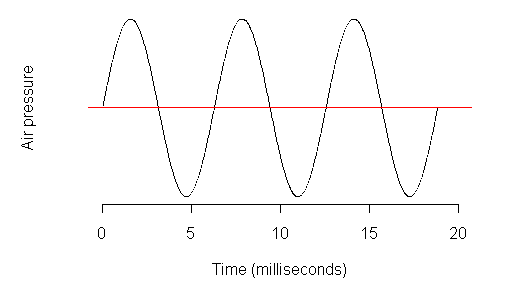
\includegraphics[width=0.7\textwidth]{figs/ln03/sound-time-pressure.png}
        \caption{Sound waves can be represented as a sequence of $({\rm time}, {\rm pressure})$ points.}
    \end{figure}
\end{center}

But actually, a large problem exists. What is ``Time''?
As in, what is ``Time'', mathematically? A set of timesteps? If so, doesn't that mean we can't detect the air pressure made by some sound in between the timesteps?
What does that question mean?
Suppose the music you listen to has one piece of sound information (one time-pressure point) sampled every 1ms starting at the 0th millisecond of a music, then what happened to the information of sound at time $1.5$ms? It simply isn't recorded.
In other words, the sound signals that we usually encounter, or listen to at the very least, are discrete, not continuous.
Discrete means that the number line our metric works on does not contain every single number; for example, if the sound signals we listen to on Spotify are sets of time-pressure points at $1ms$ intervals.
A continuous signal would be a sound signal that has the air pressure of every single granularity of seconds (in other words, for every real number worth of miliseconds, up to infinite floating point precision), which would be impossible to directly store in a computer as it contains infinite information.

As such, in computer, a sound is represented as an array of numbers.
Spotify`s sample rate, for example, is 44.1kHz. That is, 44100 time-pressure points, or samples, are beign collected per second.
This unit Hz stands for the frequency at which sampling is performed, where 1 Hz (Hertz) is equivalent to 1 cycle (of sampling) per second.

\subsection{Images}
Let us look at this following picture:
\begin{center}
    \begin{figure}[h]
        \centering
        
\includegraphics[width=0.3\textwidth]{figs/ln03/dunminghuang-grey.png}
    \end{figure}
\end{center}
Notice that this picture is made of many little squares, which we call pixels.
Every picture is made of many little pixels, and when pieced together into one large rectangular array, presents any image that we would usually see in our computer.
That means, to produce a high resolution picture, we must prepare a lot of pixels, and therefore a lot of computer storage.

For simplicity, let us represent each pixel with a number that tells us how intense the pixel's color is on a black-to-white scale (with black colors being $0$, white being $1$).
Then, suppose we have this little $20\times20$ picture above that shows a bird, then the image can be described as a signal that reports a greyscale intensity provided a target pixel:
\[
    {\rm Image}: \{1, 2, \dots, 20\} \times \{1, 2, \dots, 20\} \rightarrow \{0, \frac{1}{256}, \dots, 1\}
\]
or in a literal sense,
\[
    {\rm Image}: {\rm Horizontal} \times {\rm Vertical} \rightarrow {\rm Gresycale\ Intensity}
\]

To make the picture more colorful, we can instead represent colors as RGB triplets (Triplet of redness, greenness, and blueness of a color) in place of the original discrete greyscale intensity.
A colored version of the picture would then be a signal of the following form:
\[
    {\rm Image}: \{1, 2, \dots, 20\} \times \{1, 2, \dots, 20\} \rightarrow {\{0, \frac{1}{256}, \dots, 1\}}^3
\]
or in a literal sense,
\[
    {\rm Image}: {\rm Horizontal} \times {\rm Vertical} \rightarrow {\rm RGB\ Triplet}
\]

\subsection{Physical Attributes}
The positions of a robot device, such as a plane, can also be expressed as a signal, as they are also information that map the physical status of a device into quantifiable terms.
The easiest representation of robot positions can be a three-dimensional coordinate on Cartesian space, or a spherical coordinate with respect to Earth's center.
\[
    {\rm Position}: {\rm Time} \rightarrow \mathbb{R}^3
\]
In such way, many vector representations of physical objects that we will from now on study can also be treated as a signal.

\section{Event Stream and Sampling}
As spoken before, information are usually computationally represented as a sequence of values across specific discrete points of time and/or space.
These sequences of points that represent a signal are otherwise known as an event stream. For example, we have discussed an image as a sequence of pixel color values across the coordinates of its pixels.
For those represented information, such as the RGB triplets of pixels or pressure value of sound waves at timepoints, we call them ``symbols''.

Now that we have decided how to represent a signal in our computers discretely, we should also discuss how to obtain a discrete representation of some continuous waveform, such as an ongoing voice of violins.
In such case, let us take inspiration from our proposed form of audio storage before, that we only record 44100 samples of the violin voice each second. In such case, we measure soundwaves discretely at intervals of $\frac{1}{44100}$ seconds.
This interval at which we obtain samples of the audio is known as a sampling period.
Meanwhile, to make the pressure value (which was originally on a continuous real number line in physical world) discrete, we also let the pressure value in soundwaves be approximated to one specific number on a number line of $256$ uniformly spaced values.
All of these are examples of converting an analog signal, a signal with continuous domain and range, into a digital signal, a signal with discrete domain and range such that it may be computationally processed.


\section{Introduction to Systems}
\subsection{Definition of Systems}
Systems transform signals into other signals.
On top of that, there are a couple of things systems can do to help with this main mission:
\begin{bindenum}
    \item A system can \textbf{store} representations of some information for preservation purposes. This can later help with many other things.
    \item A system may be purposed for \textbf{transmission}, which is the delivery of one information into another system, so a system may want to preserve or transfer the information in different forms.
    \subitem In such case, a system \textbf{encodes} an information by coming up with a different representation of the original information (electronic storage of violin sounds). Meanwhile, after this component, some other system will come up with a \textbf{decoder} that decodes the information into its unencoded form.
    \subitem The encoder and decoder are together called a \textbf{codec}.
    \item A system can also instead transform a signal for the difficulty of reading (instead of making it easier to read). Or, to protect information, a machine can turn an information into another form that requires access to read. This is called \textbf{encryption}. The opposite is \textbf{decryption}.
    \item A system can also emphasize or annotate a signal to make the important parts of its information more visible. This is called \textbf{enchancing} a signal.
    \item Extraction of digital information from a signal is known as \textbf{detection}.
    \item Systems can also help \textbf{control} a specific state, such as room temperature or plane position. Such system is usually inputted the desired state via a \textbf{controller}, and collects signal to decide what to do to help with the control mission.
    \item Systems may also \textbf{translate} signals from a form into another (such as Google Translate).
\end{bindenum}

\subsection{Abstraction of Systems}
We have spoken many possible purposes of a system, a signal-to-signal function, in the above bullet points.
Then, systems can indeed be formaliezd as a function from a set of signals to another set of signals.
For example, a system $S$ that maps a signal $x$ into another output signal $y$ presents that $y = S(x)$.

Let us now concern the definition of systems at the level of not a function, but functions:
\[
    X = [D \rightarrow R] = \{x | x: D \rightarrow R\}
\]
which states that $X$, mapping from a domain $D$ to a range $R$, is the set of all $x$ that is a function mapping $D$ to $R$.
The set-builder notation is more elucidating. This set is known as a signal space, or function space.

Then, provided that systems map an input signal onto an output signal, we may discuss systems as a function whose domain and range are both signal spaces (a space of signals), such that for $y = S(x)$ and an input signal function $x$, the output signal $y$ is similarly a function that takes in some space-time related information and outputs a symbol.
Therefore, the following expression:
\[
    S(x)(z)
\]
can be interpreted as the signal (function) $y = S(x)$ taking in a space-time information $z$ and outputting the corresponding symbol or sample.

